% ============================================================
%  YatraSathi — In-Depth Beamer Presentation
%  Technical Architecture · HCI Analysis · Future Roadmap
% ============================================================
\documentclass[aspectratio=169,professionalfonts]{beamer}

\usetheme{Madrid}
\usecolortheme{default}
\setbeamercovered{transparent}
\setbeamertemplate{navigation symbols}{}
\setbeamertemplate{caption}[numbered]

% ---------- Packages ----------
\usepackage[T1]{fontenc}
\usepackage[utf8]{inputenc}
\usepackage{booktabs}
\usepackage{array}
\usepackage{amsmath}
\usepackage{tikz}
\usepackage{pgfplots}
\usepackage{hyperref}
\usepackage{tabularx}
\usepackage{colortbl}
\usepackage{multirow}
\usepackage{listings}
\usetikzlibrary{%
  arrows.meta,positioning,fit,calc,%
  shapes.geometric,shapes.symbols,%
  decorations.pathreplacing,matrix,%
  backgrounds,chains,scopes%
}
\pgfplotsset{compat=1.18}

% ---------- Colour palette (matches Flutter app) ----------
\definecolor{ysblue}{HTML}{1F4E79}
\definecolor{ysorange}{HTML}{E67E22}
\definecolor{ysgreen}{HTML}{2E8B57}
\definecolor{ysred}{HTML}{B94A48}
\definecolor{ysgray}{HTML}{5B6573}
\definecolor{yslight}{HTML}{EEF4FA}
\definecolor{yscream}{HTML}{F8F5EF}
\definecolor{ysyellow}{HTML}{F1C40F}
\definecolor{yspurple}{HTML}{7D3C98}

% ---------- Beamer theme overrides ----------
\setbeamercolor{palette primary}{bg=ysblue,fg=white}
\setbeamercolor{palette secondary}{bg=ysorange,fg=white}
\setbeamercolor{palette tertiary}{bg=ysgreen,fg=white}
\setbeamercolor{structure}{fg=ysblue}
\setbeamercolor{frametitle}{bg=yslight,fg=ysblue}
\setbeamercolor{block title}{bg=ysblue,fg=white}
\setbeamercolor{block body}{bg=yslight,fg=black}
\setbeamercolor{alertblock title}{bg=ysorange,fg=white}
\setbeamercolor{alertblock body}{bg=ysorange!10,fg=black}
\setbeamercolor{exampleblock title}{bg=ysgreen,fg=white}
\setbeamercolor{exampleblock body}{bg=ysgreen!10,fg=black}
\setbeamercolor{normal text}{fg=black,bg=white}

% ---------- Metadata ----------
\title[YatraSathi]{YatraSathi: AI-Augmented Nepal Travel Planning}
\subtitle{Architecture · HCI Analysis · Future Roadmap with Cactus Needle SLM \& RabbitMQ}
\author{Yatra Sathi Project Team}
\institute{YatraSathi Application}
\date{August 2026}

% ---------- Convenience macros ----------
\newcommand{\hl}[1]{\textbf{\textcolor{ysblue}{#1}}}
\newcommand{\hlg}[1]{\textbf{\textcolor{ysgreen}{#1}}}
\newcommand{\hlo}[1]{\textbf{\textcolor{ysorange}{#1}}}
\newcommand{\hlr}[1]{\textbf{\textcolor{ysred}{#1}}}

% ---------- TikZ style library ----------
\tikzset{
  box/.style   ={draw=ysblue,  rounded corners=3pt, thick,
                 align=center, fill=yslight,        minimum height=0.85cm, inner sep=5pt},
  box2/.style  ={draw=ysorange,rounded corners=3pt, thick,
                 align=center, fill=ysorange!12,    minimum height=0.85cm, inner sep=5pt},
  box3/.style  ={draw=ysgreen, rounded corners=3pt, thick,
                 align=center, fill=ysgreen!12,     minimum height=0.85cm, inner sep=5pt},
  box4/.style  ={draw=yspurple,rounded corners=3pt, thick,
                 align=center, fill=yspurple!10,    minimum height=0.85cm, inner sep=5pt},
  data/.style  ={draw=ysgray,  rounded corners=3pt, thick,
                 align=center, fill=gray!9,         minimum height=0.85cm, inner sep=5pt},
  slm/.style   ={draw=ysgreen, fill=ysgreen!18, rounded corners=4pt,
                 thick, align=center, minimum height=0.9cm, inner sep=6pt},
  llm/.style   ={draw=yspurple,fill=yspurple!12, rounded corners=4pt,
                 thick, align=center, minimum height=0.9cm, inner sep=6pt},
  queue/.style ={draw=ysorange,fill=ysorange!15, rounded corners=4pt,
                 thick, align=center, minimum height=0.9cm, inner sep=6pt},
  worker/.style={draw=ysblue,  fill=ysblue!10,  rounded corners=4pt,
                 thick, align=center, minimum height=0.9cm, inner sep=6pt},
  decision/.style={draw=ysblue,diamond,aspect=2.2,thick,
                   align=center,fill=yslight,inner sep=2pt},
  arrow/.style      ={-{Latex[length=2.5mm]},thick,draw=ysblue},
  arrowg/.style     ={-{Latex[length=2.5mm]},thick,draw=ysgreen},
  queuearrow/.style ={-{Latex[length=2.5mm]},thick,dashed,draw=ysorange},
  notecloud/.style  ={draw=ysgray,rounded corners,dashed,
                      fill=yscream,align=left,inner sep=5pt},
  phase/.style      ={rounded corners=3pt,minimum height=0.55cm,
                      align=center,font=\scriptsize\bfseries,text=white}
}

\begin{document}

% ============================================================
%  TITLE + TOC
% ============================================================
\begin{frame}
  \titlepage
\end{frame}

\begin{frame}{Table of Contents}
  \tableofcontents[hideallsubsections]
\end{frame}

% ============================================================
\section{Problem \& Motivation}
% ============================================================

\begin{frame}{The Problem Space}
  \begin{columns}[T]
    \column{0.54\textwidth}
    \begin{block}{Travel Planning Pain Points}
      \begin{itemize}
        \item<1-> Planning a multi-day Nepal trip requires juggling dozens of
              sources: trekking maps, food guides, accommodation listings, and
              weather data — all manually stitched together.
        \item<2-> Existing tools generate static lists.  When preferences change
              mid-planning, the user must restart from scratch.
        \item<3-> Conversational assistants produce fluent text but hide the
              decision logic, eroding user trust and control.
        \item<4-> No tool understands \emph{route geometry}: a great restaurant
              50\,km off the road is simply not useful.
      \end{itemize}
    \end{block}

    \column{0.43\textwidth}
    \begin{block}{Design Goal}
      Build a mobile-first travel planner that is
      \begin{itemize}
        \item \hl{route-aware}: recommendations stay on or near the path
        \item \hl{preference-driven}: interests, diet, pace, budget
        \item \hl{editable via chat}: natural language with inspectable results
        \item \hl{trustworthy}: every AI action is explainable and reversible
      \end{itemize}
    \end{block}
  \end{columns}
\end{frame}

\begin{frame}{Nepal as the Target Context}
  \begin{columns}[T]
    \column{0.48\textwidth}
    \begin{block}{Why Nepal is Unique}
      \begin{itemize}
        \item Complex multi-modal routes: roads, trekking trails, elevation changes
        \item High density of heterogeneous POIs: temples, viewpoints, teahouses,
              national parks, cultural heritage sites
        \item Seasonal constraints strongly affect feasibility
        \item Limited connectivity in mountain areas demands offline-ready planning
      \end{itemize}
    \end{block}

    \column{0.49\textwidth}
    \begin{alertblock}{Data Reality}
      \begin{itemize}
        \item Source: OpenStreetMap Nepal PBF (\texttt{nepal-260717.osm.pbf})
        \item Enriched via Wikidata and Wikipedia APIs
        \item 7-stage ETL pipeline normalises, deduplicates, and
              semantically tags every place record
        \item 384-dimensional embeddings (\texttt{all-MiniLM-L6-v2}) stored
              in PostgreSQL via \texttt{pgvector}
      \end{itemize}
    \end{alertblock}
  \end{columns}
\end{frame}

% ============================================================
\section{Application Overview}
% ============================================================

\begin{frame}{Application at a Glance}
  \begin{columns}[T]
    \column{0.47\textwidth}
    \begin{block}{Implemented Stack}
      \begin{itemize}
        \item \hl{Flutter} mobile app (Android / iOS / Web)
        \item \hl{FastAPI} backend with CORS, lifespan management
        \item \hl{PostgreSQL + PostGIS} for geospatial place data
        \item \hl{pgvector} extension for semantic similarity search
        \item \hl{OSRM} open-source routing engine
        \item \hl{Groq / NVIDIA NIM} LLM itinerary generation
              (\texttt{llama-3.3-70b-versatile})
        \item 7-stage \hl{ETL pipeline} from OSM PBF to production DB
      \end{itemize}
    \end{block}

    \column{0.50\textwidth}
    \begin{block}{Mobile Screens (13 total)}
      \small
      \begin{tabular}{ll}
        \texttt{home\_screen}           & Landing, quick-plan entry\\
        \texttt{explore\_screen}        & Browse places by category\\
        \texttt{plan\_screen}           & Route + trip builder\\
        \texttt{map\_screen}            & Interactive map view\\
        \texttt{place\_detail\_screen}  & Full POI detail\\
        \texttt{itinerary\_edit\_screen}& Day-by-day editor\\
        \texttt{saved\_screen}          & Saved itineraries\\
        \texttt{profile\_screen}        & User preferences\\
        \texttt{auth\_gate}             & Auth routing guard\\
      \end{tabular}
    \end{block}
  \end{columns}
\end{frame}

\begin{frame}{Current System Capabilities Summary}
  \begin{table}
    \footnotesize\centering
    \begin{tabularx}{\linewidth}{>{\bfseries}lX}
      \toprule
      Capability & Detail \\
      \midrule
      Place search    & Full-text + spatial search over PostGIS database \\
      Routing         & OSRM integration returning GeoJSON geometry, distance\_km, duration\_minutes \\
      Recommendation  & 2-stage: spatial buffer retrieval \textrightarrow\ embedding cosine scoring \textrightarrow\ trip-level optimisation \\
      Itinerary gen.  & LLM (Groq / NVIDIA NIM) from structured trip slots per pace/budget/preference \\
      Embeddings      & \texttt{all-MiniLM-L6-v2} (384-dim) via \texttt{sentence-transformers}; stored in pgvector \\
      ETL pipeline    & extract \textrightarrow\ normalize \textrightarrow\ enrich \textrightarrow\ deduplicate \textrightarrow\ semantic \textrightarrow\ embeddings \textrightarrow\ load \\
      User preferences& Interests, dietary, pace (relaxed/balanced/packed), budget (low/medium/high), family-friendly \\
      Seasonal filter & \texttt{best\_seasons} field matched against \texttt{travel\_season} query param \\
      \bottomrule
    \end{tabularx}
  \end{table}
\end{frame}

% ============================================================
\section{Technical Architecture}
% ============================================================

\begin{frame}{High-Level System Architecture}
  \begin{figure}
    \centering
    \resizebox{0.97\linewidth}{!}{%
    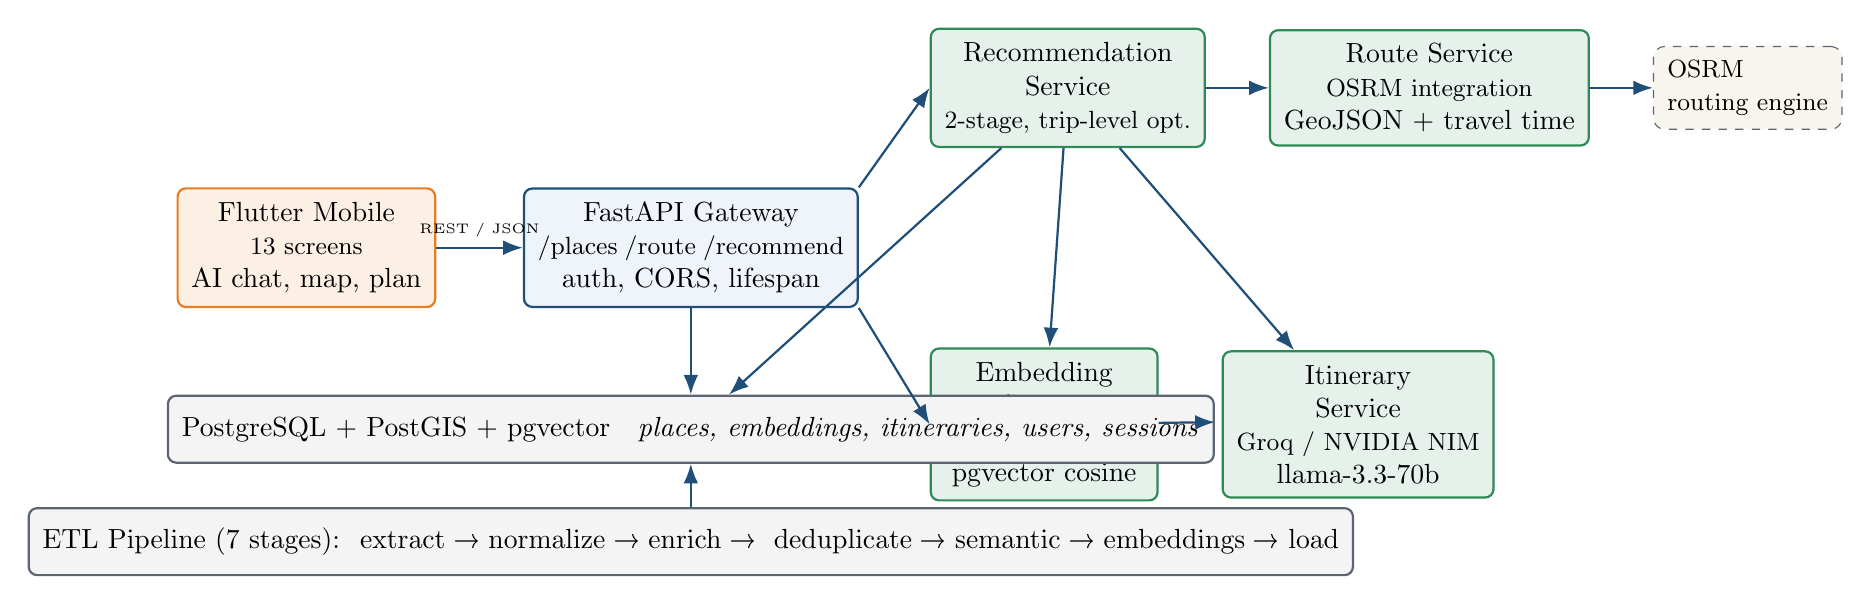
\begin{tikzpicture}[node distance=0.55cm and 0.7cm]
      % Flutter client
      \node[box2, minimum width=2.6cm] (client)
        {Flutter Mobile\\\small 13 screens\\AI chat, map, plan};

      % FastAPI
      \node[box, right=1.1cm of client, minimum width=2.8cm] (api)
        {FastAPI Gateway\\\small /places\;/route\;/recommend\\auth, CORS, lifespan};

      % Services row
      \node[box3, above right=0.5cm and 0.9cm of api, minimum width=2.6cm] (recsvc)
        {Recommendation\\Service\\\small 2-stage, trip-level opt.};
      \node[box3, right=0.8cm of recsvc, minimum width=2.6cm] (routesvc)
        {Route Service\\\small OSRM integration\\GeoJSON + travel time};
      \node[box3, below right=0.5cm and 0.9cm of api, minimum width=2.6cm] (embsvc)
        {Embedding\\Service\\\small all-MiniLM-L6-v2\\pgvector cosine};
      \node[box3, right=0.8cm of embsvc, minimum width=2.6cm] (llmsvc)
        {Itinerary\\Service\\\small Groq / NVIDIA NIM\\llama-3.3-70b};

      % DB
      \node[data, below=1.1cm of api, minimum width=5.8cm] (db)
        {PostgreSQL + PostGIS + pgvector\quad
         \textit{places, embeddings, itineraries, users, sessions}};

      % ETL
      \node[data, below=0.55cm of db, minimum width=5.8cm] (etl)
        {ETL Pipeline (7 stages):\;
         extract\;\textrightarrow\;normalize\;\textrightarrow\;enrich\;\textrightarrow\;
         deduplicate\;\textrightarrow\;semantic\;\textrightarrow\;embeddings\;\textrightarrow\;load};

      % OSRM external
      \node[notecloud, right=0.8cm of routesvc, minimum width=2.0cm] (osrm)
        {\small OSRM\\\small routing engine};

      % Arrows
      \draw[arrow] (client) -- node[above,font=\tiny]{REST / JSON} (api);
      \draw[arrow] (api.north east) -- (recsvc.west);
      \draw[arrow] (api.south east) -- (embsvc.west);
      \draw[arrow] (recsvc) -- (routesvc);
      \draw[arrow] (recsvc) -- (embsvc);
      \draw[arrow] (recsvc) -- (llmsvc);
      \draw[arrow] (routesvc) -- (osrm);
      \draw[arrow] (api) -- (db);
      \draw[arrow] (recsvc) -- (db);
      \draw[arrow] (embsvc) -- (db);
      \draw[arrow] (etl) -- (db);
    \end{tikzpicture}}
    \caption{Current implemented architecture: Flutter client, FastAPI gateway, specialised service layer, PostGIS/pgvector database, and ETL ingest pipeline.}
    \label{fig:current-arch}
  \end{figure}
\end{frame}

\begin{frame}{Database Schema}
  \begin{figure}
    \centering
    \resizebox{0.96\linewidth}{!}{%
    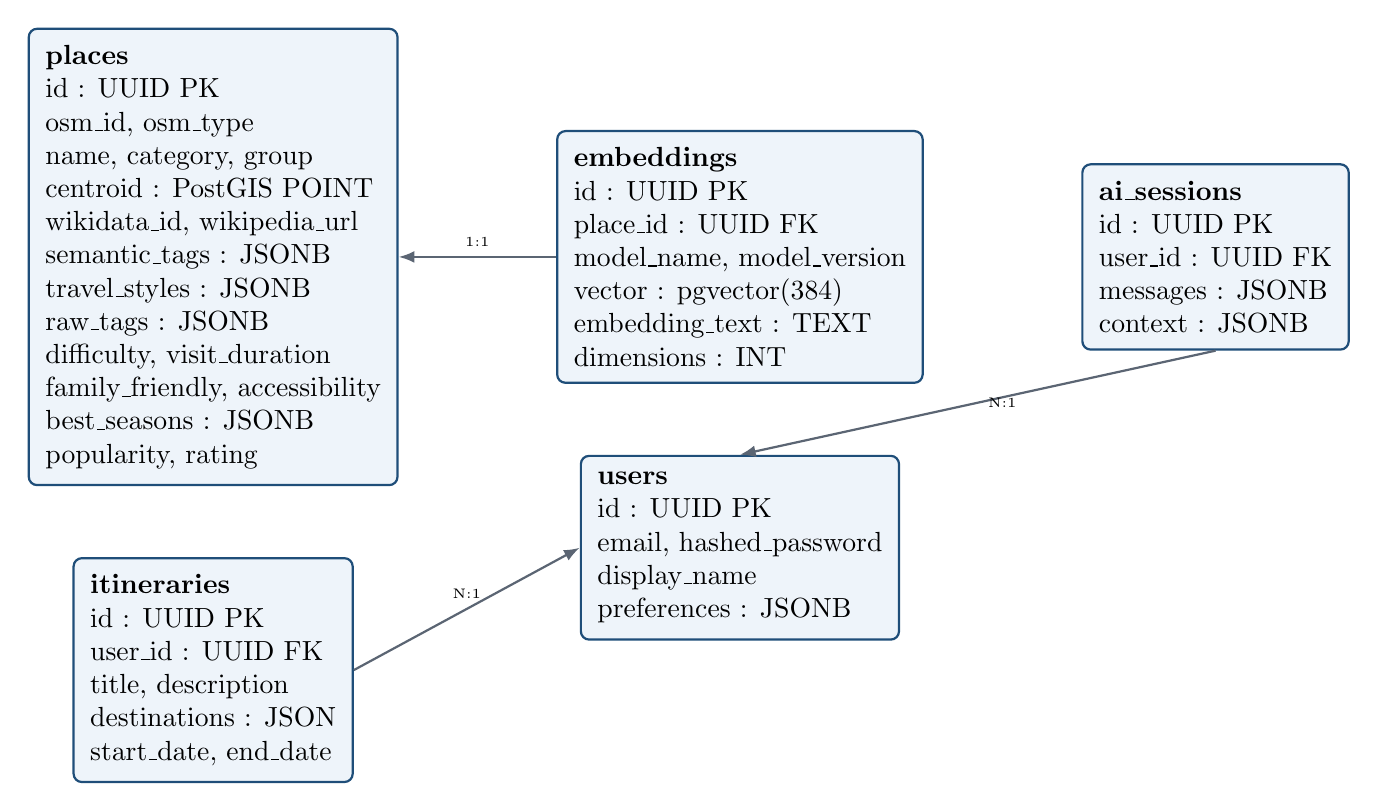
\begin{tikzpicture}[
        entity/.style={draw=ysblue,fill=yslight,rounded corners=3pt,thick,
                       align=left,inner sep=6pt,minimum width=3.0cm},
        pk/.style={font=\bfseries\scriptsize},
        fk/.style={font=\itshape\scriptsize,text=ysblue},
        attr/.style={font=\scriptsize},
        rel/.style={-{Latex[length=2mm]},thick,draw=ysgray}
      ]
      \node[entity] (places) {
        \textbf{places}\\
        \pk{id : UUID PK}\\
        \attr{osm\_id, osm\_type}\\
        \attr{name, category, group}\\
        \attr{centroid : PostGIS POINT}\\
        \attr{wikidata\_id, wikipedia\_url}\\
        \attr{semantic\_tags : JSONB}\\
        \attr{travel\_styles : JSONB}\\
        \attr{raw\_tags : JSONB}\\
        \attr{difficulty, visit\_duration}\\
        \attr{family\_friendly, accessibility}\\
        \attr{best\_seasons : JSONB}\\
        \attr{popularity, rating}
      };

      \node[entity, right=2.0cm of places] (embeddings) {
        \textbf{embeddings}\\
        \pk{id : UUID PK}\\
        \fk{place\_id : UUID FK}\\
        \attr{model\_name, model\_version}\\
        \attr{vector : pgvector(384)}\\
        \attr{embedding\_text : TEXT}\\
        \attr{dimensions : INT}
      };

      \node[entity, below=0.9cm of places] (itineraries) {
        \textbf{itineraries}\\
        \pk{id : UUID PK}\\
        \fk{user\_id : UUID FK}\\
        \attr{title, description}\\
        \attr{destinations : JSON}\\
        \attr{start\_date, end\_date}
      };

      \node[entity, below=0.9cm of embeddings] (users) {
        \textbf{users}\\
        \pk{id : UUID PK}\\
        \attr{email, hashed\_password}\\
        \attr{display\_name}\\
        \attr{preferences : JSONB}
      };

      \node[entity, right=2.0cm of embeddings] (sessions) {
        \textbf{ai\_sessions}\\
        \pk{id : UUID PK}\\
        \fk{user\_id : UUID FK}\\
        \attr{messages : JSONB}\\
        \attr{context : JSONB}
      };

      \draw[rel] (embeddings.west) -- node[above,font=\tiny]{1:1} (places.east);
      \draw[rel] (itineraries.east) -- node[above,font=\tiny]{N:1} (users.west);
      \draw[rel] (sessions.south) -- node[right,font=\tiny]{N:1} (users.north);
    \end{tikzpicture}}
    \caption{Core database schema.  The \texttt{places} table is the central entity; \texttt{embeddings} stores pgvector vectors; \texttt{itineraries} and \texttt{ai\_sessions} capture user state.}
    \label{fig:schema}
  \end{figure}
\end{frame}

\begin{frame}{ETL Pipeline: From OSM PBF to Production Embeddings}
  \begin{figure}
    \centering
    \resizebox{0.97\linewidth}{!}{%
    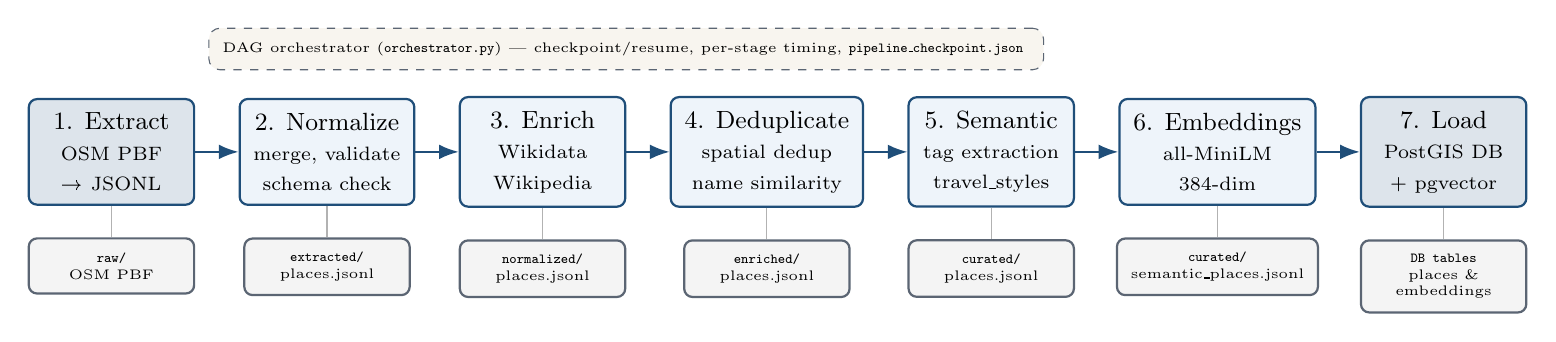
\begin{tikzpicture}[
        stage/.style={box,minimum width=2.1cm,minimum height=1.1cm,font=\small},
        file/.style={data,minimum width=2.1cm,minimum height=0.7cm,font=\tiny},
        earrow/.style={arrow}
      ]
      % Stage nodes
      \node[stage,fill=ysblue!15] (ex)   {1. Extract\\\scriptsize OSM PBF\\\scriptsize \textrightarrow\ JSONL};
      \node[stage, right=0.55cm of ex]   (no)   {2. Normalize\\\scriptsize merge, validate\\\scriptsize schema check};
      \node[stage, right=0.55cm of no]   (en)   {3. Enrich\\\scriptsize Wikidata\\\scriptsize Wikipedia};
      \node[stage, right=0.55cm of en]   (dd)   {4. Deduplicate\\\scriptsize spatial dedup\\\scriptsize name similarity};
      \node[stage, right=0.55cm of dd]   (se)   {5. Semantic\\\scriptsize tag extraction\\\scriptsize travel\_styles};
      \node[stage, right=0.55cm of se]   (emb)  {6. Embeddings\\\scriptsize all-MiniLM\\\scriptsize 384-dim};
      \node[stage, right=0.55cm of emb,fill=ysblue!15]  (ld)   {7. Load\\\scriptsize PostGIS DB\\\scriptsize + pgvector};

      % File nodes below stages
      \node[file, below=0.4cm of ex]  (raw)  {\texttt{raw/}\\OSM PBF};
      \node[file, below=0.4cm of no]  (ext)  {\texttt{extracted/}\\places.jsonl};
      \node[file, below=0.4cm of en]  (nrm)  {\texttt{normalized/}\\places.jsonl};
      \node[file, below=0.4cm of dd]  (enr)  {\texttt{enriched/}\\places.jsonl};
      \node[file, below=0.4cm of se]  (cur)  {\texttt{curated/}\\places.jsonl};
      \node[file, below=0.4cm of emb] (sem)  {\texttt{curated/}\\semantic\_places.jsonl};
      \node[file, below=0.4cm of ld]  (dbf)  {\texttt{DB tables}\\places \&\\embeddings};

      % Horizontal pipeline arrows
      \draw[earrow] (ex) -- (no);
      \draw[earrow] (no) -- (en);
      \draw[earrow] (en) -- (dd);
      \draw[earrow] (dd) -- (se);
      \draw[earrow] (se) -- (emb);
      \draw[earrow] (emb) -- (ld);

      % File connection arrows
      \foreach \s/\t in {ex/raw,no/ext,en/nrm,dd/enr,se/cur,emb/sem,ld/dbf}{
        \draw[gray!60,thin] (\s.south) -- (\t.north);
      }

      % Checkpoint banner
      \node[notecloud, above=0.35cm of no, xshift=3.8cm, minimum width=7.5cm, font=\tiny] {
        DAG orchestrator (\texttt{orchestrator.py}) — checkpoint/resume, per-stage timing, \texttt{pipeline\_checkpoint.json}
      };
    \end{tikzpicture}}
    \caption{7-stage ETL pipeline with checkpoint recovery.  Each stage reads and writes named JSONL files allowing safe resume from any failure point.}
    \label{fig:etl}
  \end{figure}
\end{frame}

\begin{frame}{Two-Stage Recommendation Engine}
  \begin{figure}
    \centering
    \resizebox{0.97\linewidth}{!}{%
    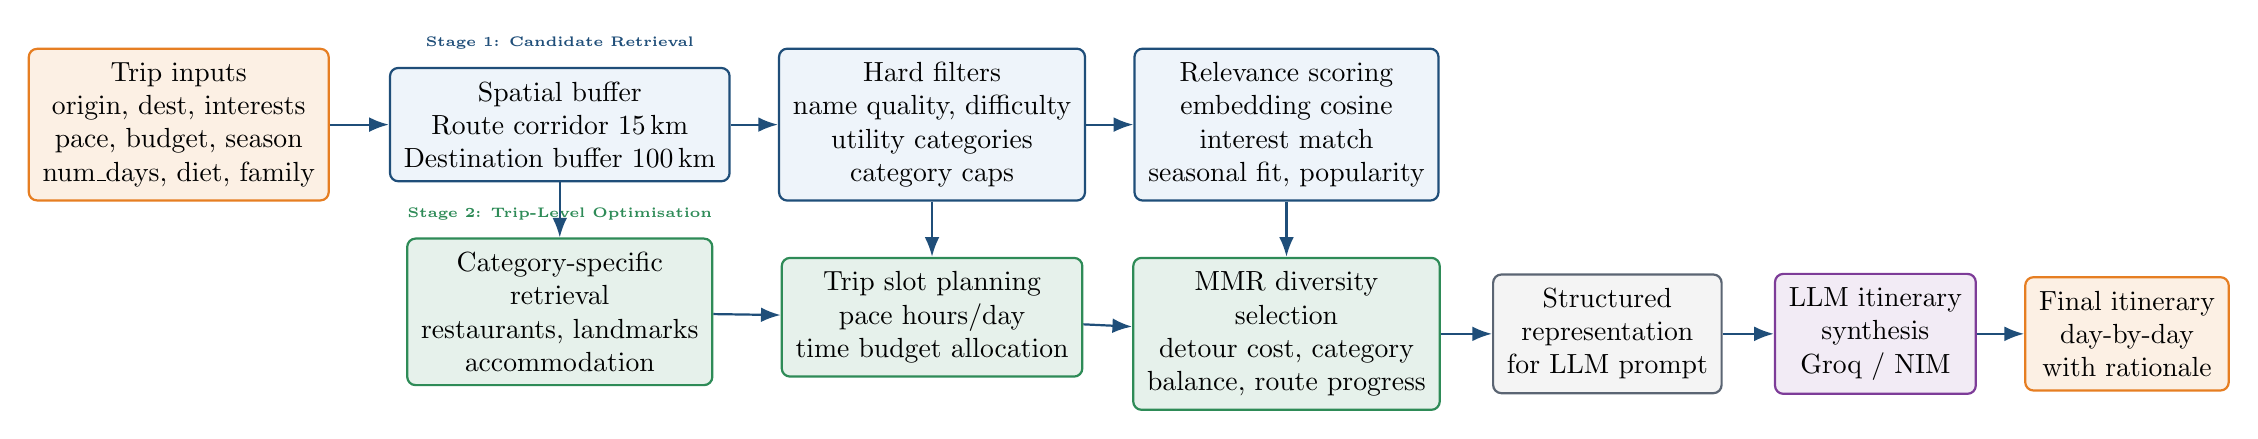
\begin{tikzpicture}[node distance=0.45cm and 0.6cm]
      % Inputs
      \node[box2, minimum width=2.5cm] (inp) {Trip inputs\\origin, dest, interests\\pace, budget, season\\num\_days, diet, family};

      % Stage 1
      \node[box, right=0.75cm of inp, minimum width=2.5cm] (spatial) {Spatial buffer\\Route corridor 15\,km\\Destination buffer 100\,km};
      \node[box, right=0.6cm of spatial, minimum width=2.5cm] (hard) {Hard filters\\name quality, difficulty\\utility categories\\category caps};
      \node[box, right=0.6cm of hard, minimum width=2.8cm] (score) {Relevance scoring\\embedding cosine\\interest match\\seasonal fit, popularity};

      % Stage 2
      \node[box3, below=0.7cm of spatial, minimum width=2.5cm] (catret) {Category-specific\\retrieval\\restaurants, landmarks\\accommodation};
      \node[box3, below=0.7cm of hard, minimum width=2.5cm] (slots) {Trip slot planning\\pace hours/day\\time budget allocation};
      \node[box3, below=0.7cm of score, minimum width=2.8cm] (mmr) {MMR diversity\\selection\\detour cost, category\\balance, route progress};

      % Outputs
      \node[data, right=0.65cm of mmr, minimum width=2.4cm] (llmin) {Structured\\representation\\for LLM prompt};
      \node[box4, right=0.65cm of llmin, minimum width=2.4cm] (llm) {LLM itinerary\\synthesis\\Groq / NIM};
      \node[box2, right=0.6cm of llm, minimum width=2.2cm] (out) {Final itinerary\\day-by-day\\with rationale};

      % Stage labels
      \node[font=\tiny\bfseries,text=ysblue, above=0.1cm of spatial] {Stage 1: Candidate Retrieval};
      \node[font=\tiny\bfseries,text=ysgreen,above=0.1cm of catret] {Stage 2: Trip-Level Optimisation};

      % Arrows stage 1
      \draw[arrow] (inp) -- (spatial);
      \draw[arrow] (spatial) -- (hard);
      \draw[arrow] (hard) -- (score);

      % Stage transition
      \draw[arrow] (score.south) -- (mmr.north);
      \draw[arrow] (spatial.south) -- (catret.north);
      \draw[arrow] (hard.south) -- (slots.north);

      % Arrows stage 2
      \draw[arrow] (catret) -- (slots);
      \draw[arrow] (slots) -- (mmr);

      % Output chain
      \draw[arrow] (mmr) -- (llmin);
      \draw[arrow] (llmin) -- (llm);
      \draw[arrow] (llm) -- (out);
    \end{tikzpicture}}
    \caption{Two-stage recommender: Stage 1 identifies relevant candidates using spatial proximity and semantic similarity; Stage 2 optimises the coherent trip set using time budget, detour cost, and diversity.}
    \label{fig:recommend}
  \end{figure}
\end{frame}

\begin{frame}{Recommendation Scoring Details}
  \begin{columns}[T]
    \column{0.48\textwidth}
    \begin{block}{Stage 1 — Candidate Scoring Signals}
      \begin{itemize}
        \item \hl{Embedding cosine similarity}: user preference vector vs.\ place vector (all-MiniLM-L6-v2)
        \item \hl{Interest keyword match}: \texttt{semantic\_tags} and \texttt{travel\_styles}
        \item \hl{Seasonal fitness}: \texttt{best\_seasons} vs.\ \texttt{travel\_season} param
        \item \hl{Popularity \& rating}: raw normalised scores from OSM/Wikidata
        \item \hl{Route proximity}: haversine distance to nearest route point
        \item \hl{Name quality score}: guards against generic or placeholder entries
      \end{itemize}
    \end{block}

    \column{0.49\textwidth}
    \begin{block}{Stage 2 — Trip-Level Optimisation}
      \begin{itemize}
        \item \hl{Pace-based time budget}: relaxed = 5h/day, balanced = 7h, packed = 9h
        \item \hl{Detour cost}: straight-line detour at 35\,km/h assumed
        \item \hl{Route progress clustering}: Day 1 = 0--33\%, Day 2 = 33--66\%, etc.
        \item \hl{Category diversity}: MMR-style re-ranking prevents flooding
        \item \hl{Hard category caps}: e.g.\ max 60 religious sites, trees = 0
        \item \hl{Family filter}: drops hard/strenuous activities when \texttt{num\_children > 0}
      \end{itemize}
    \end{block}
  \end{columns}
\end{frame}

\begin{frame}{Embedding Architecture}
  \begin{figure}
    \centering
    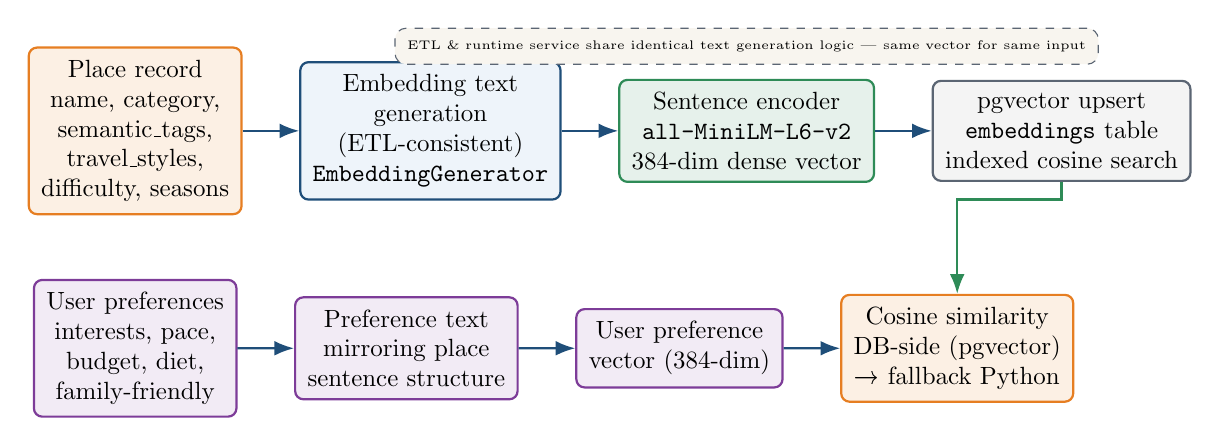
\begin{tikzpicture}[node distance=0.5cm and 0.65cm, scale=0.9, every node/.style={transform shape}]
      % Input
      \node[box2, minimum width=2.8cm] (place) {Place record\\name, category,\\semantic\_tags,\\travel\_styles,\\difficulty, seasons};

      % Text generation
      \node[box, right=0.8cm of place, minimum width=2.6cm] (txt) {Embedding text\\generation\\(ETL-consistent)\\\texttt{EmbeddingGenerator}};

      % Encode
      \node[box3, right=0.8cm of txt, minimum width=2.6cm] (enc) {Sentence encoder\\\texttt{all-MiniLM-L6-v2}\\384-dim dense vector};

      % Store
      \node[data, right=0.8cm of enc, minimum width=2.6cm] (store) {pgvector upsert\\\texttt{embeddings} table\\indexed cosine search};

      % User prefs
      \node[box4, below=0.9cm of place, minimum width=2.8cm] (pref) {User preferences\\interests, pace,\\budget, diet,\\family-friendly};
      \node[box4, right=0.8cm of pref, minimum width=2.6cm] (ptxt) {Preference text\\mirroring place\\sentence structure};
      \node[box4, right=0.8cm of ptxt, minimum width=2.6cm] (penc) {User preference\\vector (384-dim)};
      \node[box2, right=0.8cm of penc, minimum width=2.6cm] (sim)  {Cosine similarity\\DB-side (pgvector)\\\textrightarrow\ fallback Python};

      \draw[arrow] (place) -- (txt);
      \draw[arrow] (txt) -- (enc);
      \draw[arrow] (enc) -- (store);

      \draw[arrow] (pref) -- (ptxt);
      \draw[arrow] (ptxt) -- (penc);
      \draw[arrow] (penc) -- (sim);

      \draw[arrowg] (store.south) -- ++(0,-0.25) -| (sim.north);

      \node[notecloud, above=0.2cm of enc, font=\tiny] {ETL \& runtime service share identical text generation logic — same vector for same input};
    \end{tikzpicture}
    \caption{Embedding pipeline: place and user preference texts are encoded identically by the same \texttt{EmbeddingGenerator}, ensuring cosine scores are meaningful across both domains.}
    \label{fig:embedding}
  \end{figure}
\end{frame}

% ============================================================
\section{HCI Analysis}
% ============================================================

\begin{frame}{HCI Framework and Evaluation Lens}
  \begin{columns}[T]
    \column{0.49\textwidth}
    \begin{block}{Theoretical Foundations}
      \begin{itemize}
        \item \hl{Nielsen's 10 heuristics} \cite{nielsen1994}: status visibility,
              user control, error prevention, recognition over recall
        \item \hl{Shneiderman's 8 golden rules} \cite{shneiderman2016}:
              consistency, feedback, reversibility, reduced cognitive load
        \item \hl{Norman's design model} \cite{norman2013}:
              affordances, signifiers, feedback loops, conceptual model alignment
        \item \hl{Cognitive load theory} \cite{sweller2011}:
              intrinsic, extraneous, germane load management
      \end{itemize}
    \end{block}

    \column{0.48\textwidth}
    \begin{block}{Accessibility Standard}
      \begin{itemize}
        \item WCAG 2.2 \cite{wcag22} — four principles:
              \textbf{P}erceivable, \textbf{O}perable,
              \textbf{U}nderstandable, \textbf{R}obust
        \item ISO 9241-11 \cite{iso9241} — usability as
              effectiveness, efficiency, satisfaction
      \end{itemize}
    \end{block}
  \end{columns}

  \vspace{0.2cm}
  \begin{alertblock}{Central HCI Claim}
    Conversational AI itinerary editing succeeds only when it couples
    natural-language flexibility with \emph{visible state}, \emph{inspectable diffs},
    \emph{reversible actions}, and \emph{plain-language rationale}.
  \end{alertblock}
\end{frame}

\begin{frame}{User Journey Map}
  \begin{figure}
    \centering
    \resizebox{0.98\linewidth}{!}{%
    \begin{tikzpicture}
      \matrix (m) [matrix of nodes,
        nodes={draw=gray!40, minimum width=2.35cm, minimum height=0.8cm,
               align=center, font=\scriptsize, fill=white},
        column sep=-\pgflinewidth, row sep=-\pgflinewidth]{
        \cellcolor{ysblue!20}\textbf{Stage}
          & \cellcolor{ysblue!12}Discover
          & \cellcolor{ysblue!12}Plan
          & \cellcolor{ysblue!12}Generate
          & \cellcolor{ysblue!12}Review
          & \cellcolor{ysblue!12}Edit
          & \cellcolor{ysblue!12}Save / Share \\
        \textbf{Goal}
          & Find interesting\\places
          & Set route,\\filters, days
          & Get AI\\itinerary draft
          & Check fit\\and trust content
          & Adjust details\\quickly
          & Re-use or\\publish plan \\
        \textbf{Touchpoint}
          & Explore screen,\\map, search
          & Plan screen,\\route builder
          & LLM + trip\\slot pipeline
          & Proposal preview,\\route map
          & Chat widget\\+ tool actions
          & Saved screen,\\share export \\
        \textbf{Pain point}
          & Information\\overload
          & Constraint\\setup effort
          & Black-box\\AI risk
          & Fear of\\unwanted changes
          & Ambiguous\\phrasing
          & Long-term\\trust, memory \\
        \textbf{Design response}
          & Progressive\\disclosure
          & Smart defaults,\\guided input
          & Show rationale\\+ sources
          & Human approval\\gate
          & SLM tools\\+ diff preview
          & Version history\\+ provenance \\
      };

      % Emotion curve along pain point row
      \draw[ysorange,very thick,rounded corners=4pt]
        ($(m-4-2.south)+(0,-0.12)$)
        -- ++(0,-0.45)
        -- ($(m-4-3.south)+(0,-0.57)$)
        -- ++(0,-0.35)
        -- ($(m-4-4.south)+(0,-0.92)$)  % peak pain at Generate
        -- ++(0,0.35)
        -- ($(m-4-5.south)+(0,-0.57)$)  % still high at Review
        -- ++(0,0.3)
        -- ($(m-4-6.south)+(0,-0.27)$)
        -- ++(0,-0.0)
        -- ($(m-4-7.south)+(0,-0.27)$);
      \node[font=\tiny,text=ysorange] at ($(m-4-4.south)+(0,-1.15)$)
        {\small $\uparrow$ Highest trust sensitivity};
    \end{tikzpicture}}
    \caption{User journey map.  The orange emotion curve peaks at the \emph{Generate} and \emph{Review} stages, where AI opacity and fear of unwanted edits create the greatest interaction risk.}
    \label{fig:journey}
  \end{figure}
\end{frame}

\begin{frame}{Heuristic Audit of Current Interface}
  \begin{table}
    \scriptsize\centering
    \begin{tabularx}{\linewidth}{>{\bfseries}p{0.26\linewidth}
                                  >{\raggedright\arraybackslash}p{0.33\linewidth}
                                  >{\raggedright\arraybackslash}X}
      \toprule
      Heuristic & Strength in Current App & Gap / Risk \\
      \midrule
      Visibility of system status
        & Route and recommendation loading states present
        & No queue-progress indicator for long background jobs \\
      User control \& freedom
        & Proposal accept/reject flow exists
        & No global undo / redo across edit history \\
      Consistency
        & Consistent orange/cream/blue palette from \texttt{constants.dart}
        & Chat command syntax differs from button-based editing patterns \\
      Error prevention
        & Hard filters prevent nonsensical POI inclusions
        & No pre-edit impact estimate before user commits \\
      Recognition over recall
        & Categories and filters surfaced in explore screen
        & Chat interface requires user to recall available editing commands \\
      Flexibility
        & Both itinerary generation and manual place browsing supported
        & No shortcut chips for common edits (``remove last place'', etc.) \\
      Aesthetic \& minimalist design
        & Card-based place detail with progressive disclosure
        & Itinerary edit screen may overload if showing full day context \\
      \bottomrule
    \end{tabularx}
  \end{table}
\end{frame}

\begin{frame}{Cognitive Load Analysis}
  \begin{table}
    \scriptsize\centering
    \begin{tabularx}{\linewidth}{>{\bfseries}p{0.22\linewidth}
                                  >{\raggedright\arraybackslash}p{0.30\linewidth}
                                  >{\raggedright\arraybackslash}X}
      \toprule
      Load Source & Why It Matters & Mitigation Strategy \\
      \midrule
      Intent formulation
        & Translating travel goals into edit commands is effortful
        & Suggestion chips, contextual command hints, SLM slot-filling \\
      State tracking
        & Users forget what changed across multi-turn edits
        & Persistent diff summary, version labels, undo stack \\
      Consequence prediction
        & Edits silently affect time budget, route, balance
        & Surface impact estimates (time delta, cost estimate) before approval \\
      Trust calibration
        & Users cannot distinguish deterministic vs.\ generative results
        & Label each result: \emph{tool action} vs.\ \emph{AI generated} \\
      Recovery effort
        & Failed commands leave uncertain system state
        & Explicit error cards, no-op recovery messages, state restoration \\
      Information overload
        & Nepal has thousands of POIs; exploration can overwhelm
        & Progressive disclosure: overview \textrightarrow\ category \textrightarrow\ detail \\
      \bottomrule
    \end{tabularx}
  \end{table}
  \vspace{0.1cm}
  \begin{exampleblock}{Design Principle}
    The interface must carry the bookkeeping burden so the traveller can stay
    in creative planning mode.
  \end{exampleblock}
\end{frame}

\begin{frame}{Chat Interface Interaction Model}
  \begin{figure}
    \centering
    \resizebox{0.97\linewidth}{!}{%
    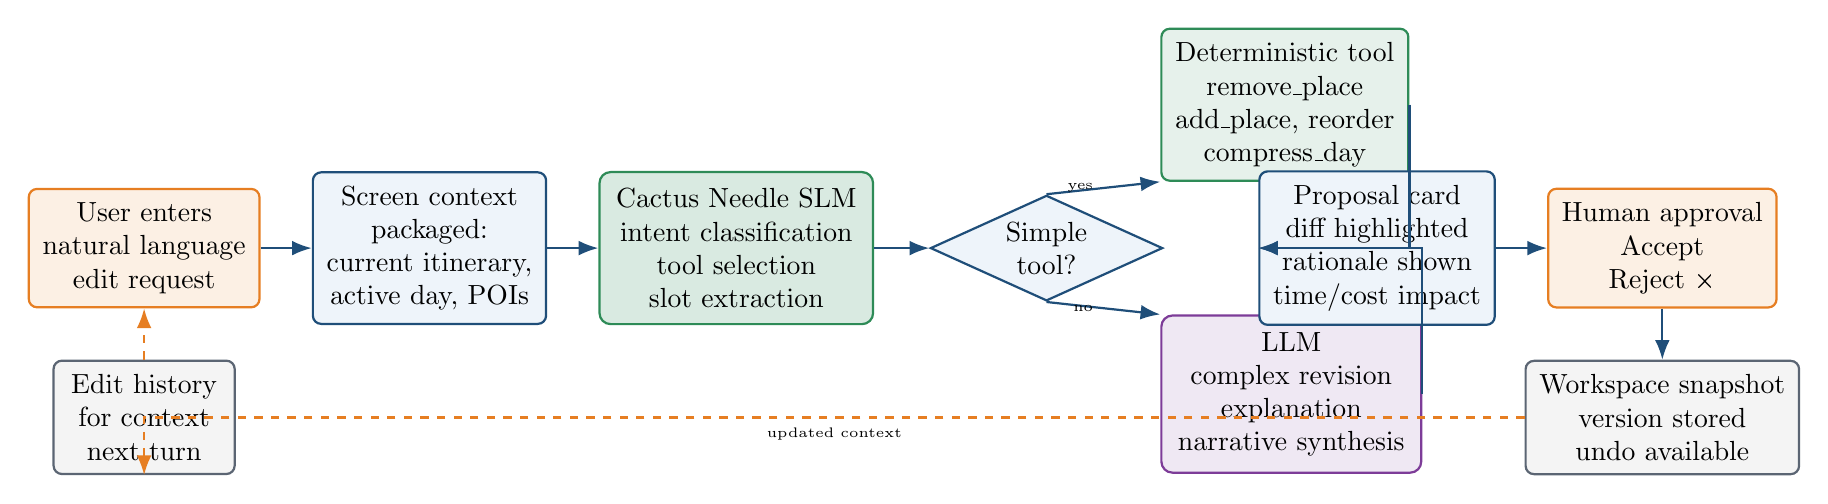
\begin{tikzpicture}[node distance=0.38cm and 0.55cm]
      \node[box2, minimum width=2.2cm] (input)
        {User enters\\natural language\\edit request};
      \node[box, right=0.65cm of input, minimum width=2.3cm] (ctx)
        {Screen context\\packaged:\\current itinerary,\\active day, POIs};
      \node[slm, right=0.65cm of ctx, minimum width=2.3cm] (slm)
        {Cactus Needle SLM\\intent classification\\tool selection\\slot extraction};
      \node[decision, right=0.7cm of slm] (dec)
        {Simple\\tool?};

      \node[box3, above right=0.5cm and 0.7cm of dec, minimum width=2.2cm] (tools)
        {Deterministic tool\\remove\_place\\add\_place, reorder\\compress\_day};
      \node[llm,  below right=0.5cm and 0.7cm of dec, minimum width=2.2cm] (llm)
        {LLM\\complex revision\\explanation\\narrative synthesis};
      \node[box,  right=1.2cm of dec, minimum width=2.3cm] (prop)
        {Proposal card\\diff highlighted\\rationale shown\\time/cost impact};
      \node[box2, right=0.65cm of prop, minimum width=2.2cm] (gate)
        {Human approval\\Accept \checkmark\\Reject \texttimes};
      \node[data, below=0.65cm of gate, minimum width=2.3cm] (ws)
        {Workspace snapshot\\version stored\\undo available};
      \node[data, below=0.65cm of input, minimum width=2.3cm] (hist)
        {Edit history\\for context\\next turn};

      \draw[arrow] (input) -- (ctx);
      \draw[arrow] (ctx)   -- (slm);
      \draw[arrow] (slm)   -- (dec);
      \draw[arrow] (dec.north) -- node[left,font=\tiny]{yes} (tools.south west);
      \draw[arrow] (dec.south) -- node[left,font=\tiny]{no}  (llm.north west);
      \draw[arrow] (tools.east) |- (prop.west);
      \draw[arrow] (llm.east)   |- (prop.west);
      \draw[arrow] (prop)  -- (gate);
      \draw[arrow] (gate)  -- (ws);
      \draw[queuearrow] (ws.west) -| node[pos=0.25,below,font=\tiny]{updated context} (hist.south);
      \draw[queuearrow] (hist.north) -- (input.south);
    \end{tikzpicture}}
    \caption{Chat-based editing flow.  The SLM routes simple, structured edits to deterministic tools while complex or ambiguous requests escalate to the LLM.  Every output passes through a human approval gate before the workspace is modified.}
    \label{fig:chatflow}
  \end{figure}
\end{frame}

\begin{frame}{Accessibility and Inclusive Design}
  \begin{columns}[T]
    \column{0.48\textwidth}
    \begin{block}{WCAG 2.2 Requirements}
      \begin{itemize}
        \item \hl{Perceivable}: APCA-compliant contrast on orange/blue palette;
              non-colour proposal status indicators; alt-text for map exports
        \item \hl{Operable}: large tap targets ($\geq$44\,dp);
              keyboard-accessible controls; timeout-free approval flows
        \item \hl{Understandable}: plain-language action descriptions;
              localised Nepali/English date formatting; jargon-free errors
        \item \hl{Robust}: semantic widget structure in Flutter;
              screen-reader state announcements for proposal and queue events
      \end{itemize}
    \end{block}

    \column{0.49\textwidth}
    \begin{alertblock}{Real-World Constraints}
      Nepal travel planning happens in conditions that intensify accessibility needs:
      \begin{itemize}
        \item Low-bandwidth mountain connectivity \textrightarrow\ offline-first
              data caching
        \item Bright sunlight \textrightarrow\ high-contrast mode
        \item One-handed use while navigating \textrightarrow\ large, single-tap
              confirm/reject
        \item Multilingual group travel \textrightarrow\ localisation support
      \end{itemize}
    \end{alertblock}
  \end{columns}
\end{frame}

\begin{frame}{Usability Evaluation Protocol}
  \begin{columns}[T]
    \column{0.50\textwidth}
    \begin{block}{Study Methods}
      \begin{itemize}
        \item Moderated think-aloud sessions (6--8 participants per cohort)
        \item Task-based benchmark: edit completion time, error rate
        \item NASA-TLX workload survey post-task
        \item Post-session confidence interview
        \item In-app telemetry: approval rate, revert rate, re-edit frequency,
              drop-off points
      \end{itemize}
    \end{block}

    \column{0.47\textwidth}
    \begin{block}{Benchmark Tasks}
      \begin{enumerate}
        \item Remove a place and preserve trip duration
        \item Add a low-effort alternative near the route
        \item Compare and approve two proposed revisions
        \item Recover from a failed or ambiguous edit command
        \item Plan a 3-day trip from Kathmandu to Pokhara end-to-end
      \end{enumerate}
    \end{block}
  \end{columns}

  \vspace{0.18cm}
  \begin{exampleblock}{Primary Metrics \cite{lazar2017,dumas1999,iso9241}}
    Task success rate $\cdot$ Time on task $\cdot$ Approval confidence score $\cdot$
    Error recovery rate $\cdot$ Re-edit frequency $\cdot$ Perceived workload (NASA-TLX)
  \end{exampleblock}
\end{frame}

% ============================================================
\section{Future Plans}
% ============================================================

\begin{frame}{Future Architecture: Target State}
  \begin{figure}
    \centering
    \resizebox{0.98\linewidth}{!}{%
    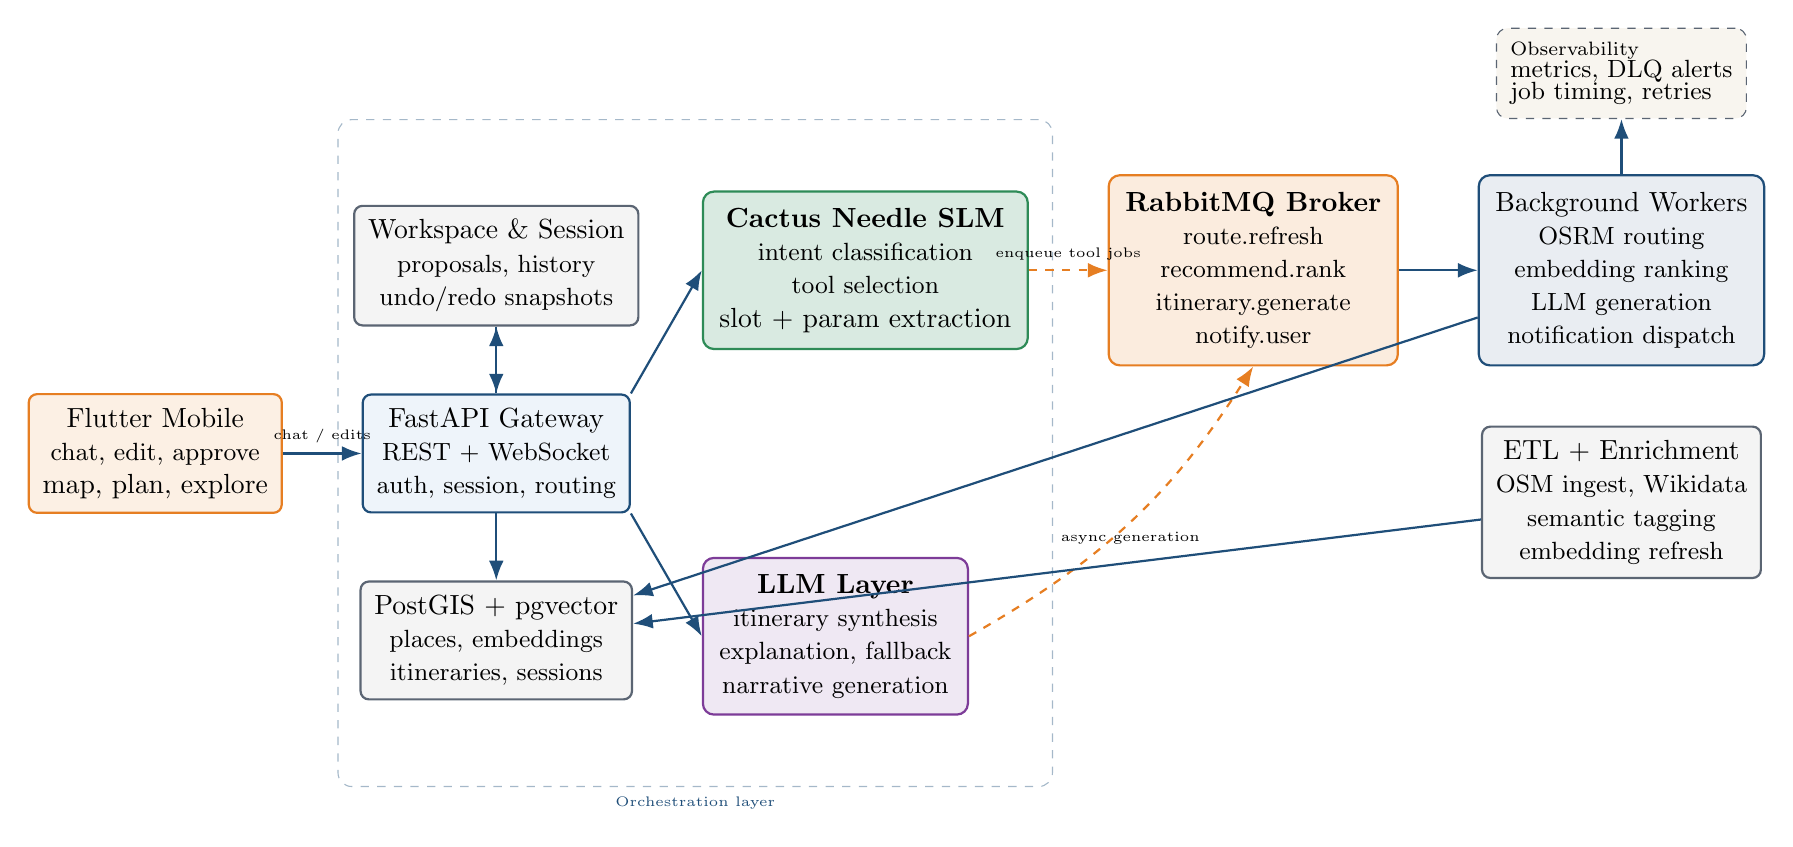
\begin{tikzpicture}[node distance=0.52cm and 0.65cm]
      % Flutter
      \node[box2, minimum width=2.7cm] (client)
        {Flutter Mobile\\\small chat, edit, approve\\map, plan, explore};

      % API
      \node[box, right=1.0cm of client, minimum width=2.8cm] (api)
        {FastAPI Gateway\\\small REST + WebSocket\\\small auth, session, routing};

      % SLM
      \node[slm, above right=0.55cm and 0.9cm of api, minimum width=2.9cm] (slm)
        {\textbf{Cactus Needle SLM}\\\small intent classification\\\small tool selection\\slot + param extraction};

      % LLM
      \node[llm, below right=0.55cm and 0.9cm of api, minimum width=2.9cm] (llm)
        {\textbf{LLM Layer}\\\small itinerary synthesis\\\small explanation, fallback\\\small narrative generation};

      % Workspace state
      \node[data, above=0.85cm of api, minimum width=2.7cm] (ws)
        {Workspace \& Session\\\small proposals, history\\\small undo/redo snapshots};

      % DB
      \node[data, below=0.85cm of api, minimum width=2.7cm] (db)
        {PostGIS + pgvector\\\small places, embeddings\\\small itineraries, sessions};

      % RabbitMQ
      \node[queue, right=1.0cm of slm, minimum width=3.0cm] (rmq)
        {\textbf{RabbitMQ Broker}\\\small route.refresh\\\small recommend.rank\\\small itinerary.generate\\\small notify.user};

      % Workers
      \node[worker, right=1.0cm of rmq, minimum width=2.8cm] (workers)
        {Background Workers\\\small OSRM routing\\\small embedding ranking\\\small LLM generation\\\small notification dispatch};

      % ETL
      \node[data, below=0.75cm of workers, minimum width=2.8cm] (etl)
        {ETL + Enrichment\\\small OSM ingest, Wikidata\\\small semantic tagging\\\small embedding refresh};

      % Observability
      \node[notecloud, above=0.7cm of workers, minimum width=2.8cm, font=\scriptsize] (obs)
        {Observability\\\small metrics, DLQ alerts\\\small job timing, retries};

      % Arrows
      \draw[arrow]      (client) -- node[above,font=\tiny]{chat / edits} (api);
      \draw[arrow]      (api.north east) -- (slm.west);
      \draw[arrow]      (api.south east) -- (llm.west);
      \draw[arrow]      (ws) -- (api);
      \draw[arrow]      (api) -- (db);
      \draw[queuearrow] (slm.east) -- node[above,font=\tiny]{enqueue tool jobs} (rmq.west);
      \draw[queuearrow] (llm.east) to[bend right=14] node[below,font=\tiny]{async generation} (rmq.south);
      \draw[arrow]      (rmq) -- (workers);
      \draw[arrow]      (workers) -- (db);
      \draw[arrow]      (etl) -- (db);
      \draw[arrow]      (workers) -- (obs);
      \draw[arrow]      (api) -- (ws);

      % Boundary box
      \begin{pgfonlayer}{background}
        \node[draw=ysblue!40,dashed,rounded corners=5pt,
              fit=(api)(slm)(llm),
              inner ysep=0.9cm, inner xsep=0.3cm,
              label={[font=\tiny,text=ysblue]below:Orchestration layer}] {};
      \end{pgfonlayer}
    \end{tikzpicture}}
    \caption{Target-state architecture adding Cactus Needle SLM intent routing, RabbitMQ-backed asynchronous worker pools, and improved workspace state management.}
    \label{fig:future-arch}
  \end{figure}
\end{frame}

\begin{frame}{Cactus Needle SLM: Role and Rationale}
  \begin{columns}[T]
    \column{0.50\textwidth}
    \begin{block}{What Cactus Needle Does}
      \begin{itemize}
        \item \hl{Intent classification}: is the user requesting an edit,
              a query, navigation, or information?
        \item \hl{Tool selection}: maps intent to one or more of the
              defined editing tools
        \item \hl{Slot extraction}: resolves entity references
              (``the museum'' \textrightarrow\ matched place ID)
        \item \hl{Parameter validation}: checks extracted slots against
              schema before any tool call
        \item \hl{Fallback signal}: low-confidence \textrightarrow\ escalate
              to LLM with context
      \end{itemize}
    \end{block}

    \column{0.47\textwidth}
    \begin{block}{Why Not Always Use LLM?}
      \begin{itemize}
        \item LLM calls add 1--4\,s latency for edits that can be
              resolved deterministically in $<$200\,ms
        \item SLMs are smaller, faster, cheaper to host, and easier to
              audit for compliance
        \item Deterministic tool paths are fully testable; LLM paths
              have stochastic output
        \item Model allocation: LLM reserved for \emph{creative synthesis}
              and \emph{ambiguity resolution} only
      \end{itemize}
    \end{block}
  \end{columns}

  \vspace{0.18cm}
  \begin{alertblock}{Key Principle}
    Cactus Needle is a \emph{controller}, not an author.
    It turns natural language into structured, validated operations.
    The LLM turns structured context into readable, trustworthy narratives.
  \end{alertblock}
\end{frame}

\begin{frame}{SLM-Enhanced Editing Tool Workflow}
  \begin{figure}
    \centering
    \resizebox{0.97\linewidth}{!}{%
    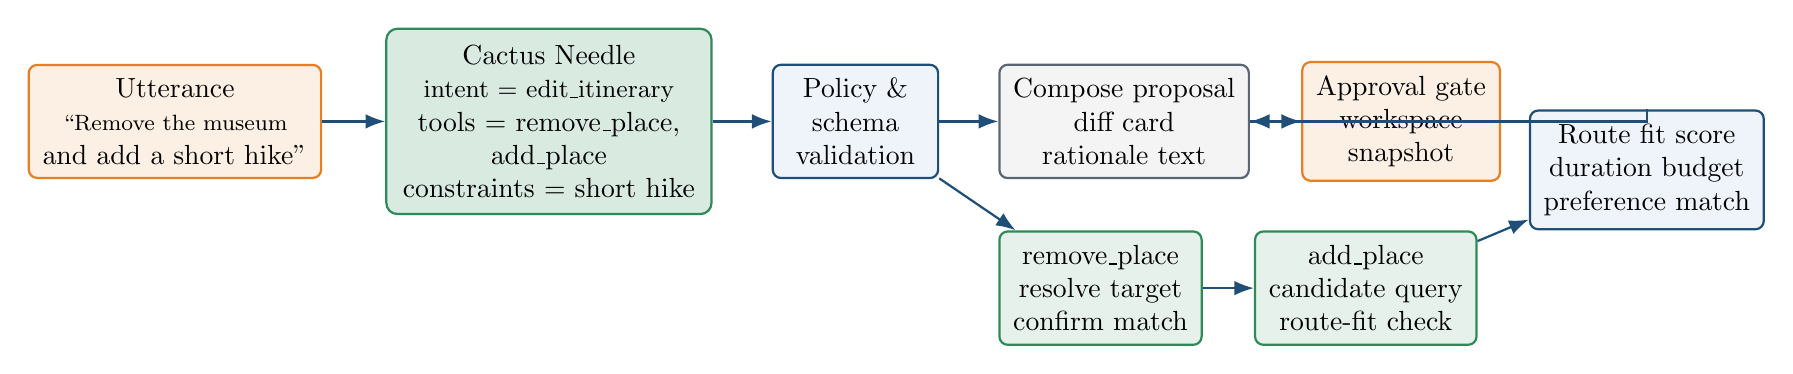
\begin{tikzpicture}[node distance=0.42cm and 0.6cm]
      \node[box2, minimum width=2.1cm] (utt)
        {Utterance\\\footnotesize``Remove the museum\\and add a short hike''};
      \node[slm, right=0.8cm of utt, minimum width=2.6cm] (parse)
        {Cactus Needle\\\small intent = edit\_itinerary\\tools = remove\_place,\\add\_place\\constraints = short hike};
      \node[box, right=0.75cm of parse, minimum width=2.1cm] (policy)
        {Policy \&\\schema\\validation};

      \node[box3, below right=0.65cm and 0.75cm of policy, minimum width=2.1cm] (rm)
        {remove\_place\\resolve target\\confirm match};
      \node[box3, right=0.65cm of rm, minimum width=2.1cm] (add)
        {add\_place\\candidate query\\route-fit check};
      \node[box, above right=0.0cm and 0.65cm of add, minimum width=2.3cm] (score)
        {Route fit score\\duration budget\\preference match};
      \node[data, right=0.75cm of policy, minimum width=2.2cm] (diff)
        {Compose proposal\\diff card\\rationale text};
      \node[box2, right=0.65cm of diff, minimum width=2.0cm] (gate)
        {Approval gate\\workspace\\snapshot};

      \draw[arrow] (utt)    -- (parse);
      \draw[arrow] (parse)  -- (policy);
      \draw[arrow] (policy) -- (rm);
      \draw[arrow] (rm)     -- (add);
      \draw[arrow] (add)    -- (score);
      \draw[arrow] (score.north) |- (diff.east);
      \draw[arrow] (policy) -- (diff);
      \draw[arrow] (diff)   -- (gate);
    \end{tikzpicture}}
    \caption{Cactus Needle decomposes a compound utterance into two sequenced tool calls.  Rule-based scorers evaluate route fit and duration constraints before the proposal reaches the user.}
    \label{fig:slmworkflow}
  \end{figure}
\end{frame}

\begin{frame}{Defined SLM Editing Tools (Tool API)}
  \begin{table}
    \footnotesize\centering
    \begin{tabularx}{\linewidth}{>{\bfseries\ttfamily}p{0.22\linewidth}
                                  >{\raggedright\arraybackslash}p{0.28\linewidth}
                                  >{\raggedright\arraybackslash}X}
      \toprule
      Tool Name & Input Slots & Backend Logic \\
      \midrule
      remove\_place
        & place\_id or name, day
        & Resolve by name similarity, validate day membership, remove from slot \\
      add\_place
        & category, constraints, target\_day
        & Query candidates by embedding + filters, score route fit, select best \\
      reorder\_places
        & day, from\_index, to\_index
        & Validate indices, swap positions, re-check time budget \\
      swap\_place
        & old\_place\_id, constraints
        & Find alternative via embedding search, preserve time slot \\
      compress\_day
        & day, target\_hours
        & Drop lowest-priority places until daily time budget met \\
      expand\_day
        & day, extra\_hours
        & Add candidates from scored pool respecting category diversity \\
      budget\_replace
        & day, budget\_level
        & Replace above-budget POIs with scored lower-cost alternatives \\
      \bottomrule
    \end{tabularx}
  \end{table}
  \vspace{0.05cm}
  \scriptsize Launch scope: \texttt{remove\_place} and \texttt{add\_place}.
  Remaining tools added iteratively each quarter.
\end{frame}

\begin{frame}{RabbitMQ Background Processing Architecture}
  \begin{columns}[T]
    \column{0.47\textwidth}
    \begin{block}{Queue Topology}
      \begin{itemize}
        \item \texttt{route.refresh} — OSRM routing jobs; re-computed on trip parameter change
        \item \texttt{recommend.rank} — spatial buffer + embedding ranking jobs
        \item \texttt{itinerary.generate} — LLM itinerary synthesis (long-running)
        \item \texttt{notify.user} — push WebSocket or mobile notification on completion
        \item \texttt{*.dlq} — dead-letter queues with retry-with-backoff
      \end{itemize}
    \end{block}

    \column{0.50\textwidth}
    \begin{block}{Reliability Controls}
      \begin{itemize}
        \item \hl{Idempotency keys}: same request never produces duplicate jobs
        \item \hl{At-least-once delivery}: worker acknowledges only on success
        \item \hl{Dead-letter routing}: failed jobs inspectable, re-queueable
        \item \hl{Backoff policy}: 1\,s, 5\,s, 30\,s retries before DLQ
        \item \hl{Queue monitoring}: job rate, depth, DLQ alerts
        \item \hl{Worker autoscaling}: horizontal pods per queue depth threshold
      \end{itemize}
    \end{block}
  \end{columns}
\end{frame}

\begin{frame}{RabbitMQ Sequence Diagram}
  \begin{figure}
    \centering
    \resizebox{0.97\linewidth}{!}{%
    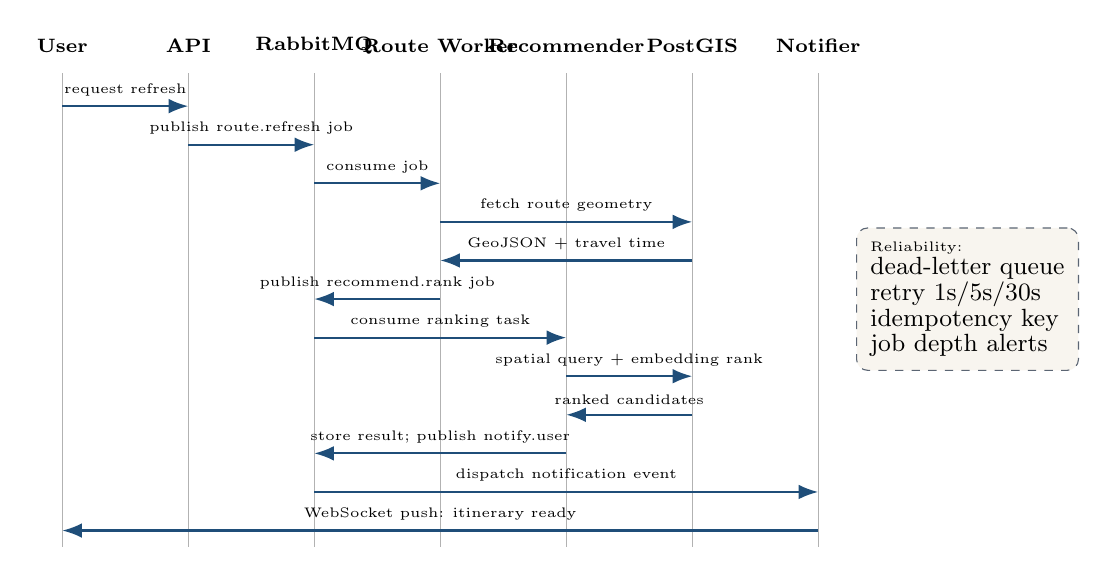
\begin{tikzpicture}[x=1.6cm, y=0.70cm]
      % Lifelines
      \foreach \i/\name in {%
          0/User,
          1/API,
          2/{RabbitMQ},
          3/{Route Worker},
          4/{Recommender},
          5/{PostGIS},
          6/{Notifier}}{
        \node[font=\scriptsize\bfseries] at (\i, 0.3) {\name};
        \draw[gray!60, thin] (\i,-0.2) -- (\i,-8.8);
      }

      % Messages
      \draw[arrow] (0,-0.8)  -- node[above,font=\tiny]{request refresh} (1,-0.8);
      \draw[arrow] (1,-1.5)  -- node[above,font=\tiny]{publish route.refresh job} (2,-1.5);
      \draw[arrow] (2,-2.2)  -- node[above,font=\tiny]{consume job} (3,-2.2);
      \draw[arrow] (3,-2.9)  -- node[above,font=\tiny]{fetch route geometry} (5,-2.9);
      \draw[arrow] (5,-3.6)  -- node[above,font=\tiny]{GeoJSON + travel time} (3,-3.6);
      \draw[arrow] (3,-4.3)  -- node[above,font=\tiny]{publish recommend.rank job} (2,-4.3);
      \draw[arrow] (2,-5.0)  -- node[above,font=\tiny]{consume ranking task} (4,-5.0);
      \draw[arrow] (4,-5.7)  -- node[above,font=\tiny]{spatial query + embedding rank} (5,-5.7);
      \draw[arrow] (5,-6.4)  -- node[above,font=\tiny]{ranked candidates} (4,-6.4);
      \draw[arrow] (4,-7.1)  -- node[above,font=\tiny]{store result; publish notify.user} (2,-7.1);
      \draw[arrow] (2,-7.8)  -- node[above,font=\tiny]{dispatch notification event} (6,-7.8);
      \draw[arrow] (6,-8.5)  -- node[above,font=\tiny]{WebSocket push: itinerary ready} (0,-8.5);

      % Reliability callout
      \node[notecloud, anchor=north west, font=\tiny] at (6.3,-3.0) {
        Reliability:\\\small dead-letter queue\\\small retry 1s/5s/30s\\\small idempotency key\\\small job depth alerts
      };
    \end{tikzpicture}}
    \caption{RabbitMQ-backed routing and recommendation refresh sequence.  The Flutter UI receives a WebSocket push only when results are ready, keeping the conversational interface non-blocking.}
    \label{fig:rabbitmq}
  \end{figure}
\end{frame}

\begin{frame}{LLM Strategy and Model Allocation}
  \begin{columns}[T]
    \column{0.50\textwidth}
    \begin{block}{Reserved for LLM}
      \begin{itemize}
        \item Initial multi-day itinerary synthesis from structured trip slots
        \item Natural-language rationale for recommendation choices
        \item Ambiguity resolution when SLM confidence is below threshold
        \item Complex conversational editing (``redesign Day 2 around heritage'')
        \item Explanation of trade-offs (time, cost, difficulty, route detour)
      \end{itemize}
    \end{block}

    \column{0.47\textwidth}
    \begin{block}{Model Selection Criteria}
      \begin{itemize}
        \item \hl{Instruction fidelity}: follows structured JSON schema output
        \item \hl{Latency}: acceptable p95 for background queue jobs
        \item \hl{Cost}: per-token cost within monthly budget envelope
        \item \hl{Controllability}: temperature, max tokens, stop sequences
        \item \hl{Provider diversity}: Groq and NVIDIA NIM as current options;
              abstracted via provider interface for easy swap
      \end{itemize}
    \end{block}
  \end{columns}

  \vspace{0.15cm}
  \begin{exampleblock}{Anti-Hallucination Constraints (already implemented)}
    LLM prompts include explicit instructions: only use provided POI list,
    never fabricate place names, output strict JSON schema,
    reject if fewer candidates than days.
  \end{exampleblock}
\end{frame}

\begin{frame}{Current vs.\ Future: Baseline--Delta Table}
  \begin{table}
    \footnotesize\centering
    \begin{tabularx}{\linewidth}{>{\bfseries}p{0.22\linewidth}
                                  >{\raggedright\arraybackslash}p{0.32\linewidth}
                                  >{\raggedright\arraybackslash}X}
      \toprule
      Layer & Current Baseline & Proposed Extension \\
      \midrule
      Client interaction
        & Chat widget, proposal review, map, itinerary edit
        & Edit chips, diff cards, queue-progress states, SLM-labelled actions \\
      AI orchestration
        & Direct LLM itinerary generation
        & Cactus Needle SLM for intent routing; LLM reserved for synthesis \\
      Background execution
        & Synchronous request/response (blocking)
        & RabbitMQ queues for routing, ranking, generation, notifications \\
      State management
        & Session records (SQLAlchemy \texttt{ai\_sessions})
        & Workspace snapshots, undo stack, durable proposal history \\
      Editing tools
        & Manual itinerary edit screen (UI only)
        & remove\_place, add\_place, reorder, swap, compress, expand, budget\_replace \\
      Scalability
        & Single-service orchestration path
        & Horizontal worker pools per queue with autoscaling \\
      Observability
        & Application logs
        & Queue metrics, DLQ monitoring, job timing, recommendation anomaly detection \\
      \bottomrule
    \end{tabularx}
  \end{table}
\end{frame}

\begin{frame}{Phased Development Roadmap}
  \begin{figure}
    \centering
    \resizebox{0.97\linewidth}{!}{%
    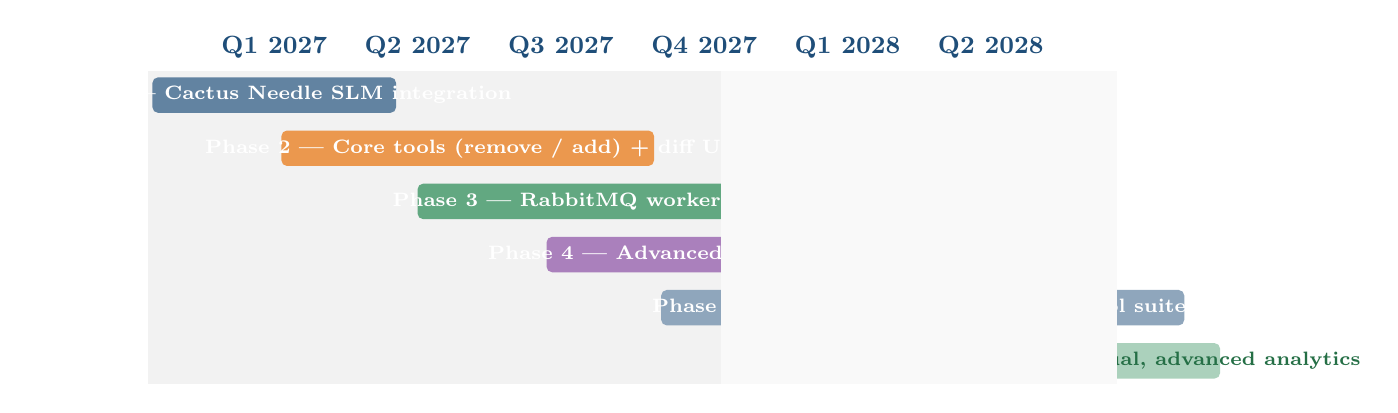
\begin{tikzpicture}[x=1.82cm, y=0.75cm]
      % Quarter headers
      \foreach \x/\lbl in {0/Q1 2027, 1/Q2 2027, 2/Q3 2027, 3/Q4 2027}{
        \node[font=\small\bfseries,text=ysblue] at (\x+0.9, 5.7) {\lbl};
        \fill[gray!10] (\x+0.02,0) rectangle (\x+1.78,5.3);
      }

      % Phase bars (start_x, start_y, width, height, colour, label)
      % Phase 1 — SLM integration
      \fill[ysblue!70,rounded corners=2pt] (0.05,4.6) rectangle (1.75,5.2);
      \node[font=\scriptsize\bfseries,text=white] at (0.9,4.9)
        {Phase 1 — Cactus Needle SLM integration};

      % Phase 2 — Core editing tools + diff UI
      \fill[ysorange!80,rounded corners=2pt] (0.95,3.7) rectangle (3.55,4.3);
      \node[font=\scriptsize\bfseries,text=white] at (2.25,4.0)
        {Phase 2 — Core tools (remove / add) + diff UI};

      % Phase 3 — RabbitMQ background workers
      \fill[ysgreen!75,rounded corners=2pt] (1.9,2.8) rectangle (4.35,3.4);
      \node[font=\scriptsize\bfseries,text=white] at (3.1,3.1)
        {Phase 3 — RabbitMQ worker pools};

      % Phase 4 — Advanced tools + research validation
      \fill[yspurple!65,rounded corners=2pt] (2.8,1.9) rectangle (5.65,2.5);
      \node[font=\scriptsize\bfseries,text=white] at (4.22,2.2)
        {Phase 4 — Advanced tools + usability research};

      % Phase 5 — Scale-out + accessibility + full tool suite
      \fill[ysblue!50,rounded corners=2pt] (3.6,1.0) rectangle (7.25,1.6);
      \node[font=\scriptsize\bfseries,text=white] at (5.4,1.3)
        {Phase 5 — Scale-out, accessibility, full tool suite};

      % Beyond — continuous improvement
      \fill[ysgreen!40,rounded corners=2pt] (5.5,0.1) rectangle (7.5,0.7);
      \node[font=\scriptsize\bfseries,text=ysgreen!80!black] at (6.5,0.4)
        {Phase 6 — Offline, multilingual, advanced analytics};

      % X-axis extension for phase 5+6
      \foreach \x/\lbl in {4/Q1 2028, 5/Q2 2028}{
        \node[font=\small\bfseries,text=ysblue] at (\x+0.9, 5.7) {\lbl};
        \fill[gray!5] (\x+0.02,0) rectangle (\x+1.78,5.3);
      }
    \end{tikzpicture}}
    \caption{Phased roadmap across 6 development phases.  Phases are cumulative: each builds on a validated foundation before expanding scope.}
    \label{fig:timeline}
  \end{figure}
\end{frame}

\begin{frame}{Milestones, Dependencies, and Success Metrics}
  \begin{table}
    \scriptsize\centering
    \begin{tabularx}{\linewidth}{>{\bfseries}p{0.18\linewidth}
                                  >{\raggedright\arraybackslash}p{0.27\linewidth}
                                  >{\raggedright\arraybackslash}X}
      \toprule
      Milestone & Critical Dependencies & Success Metrics \\
      \midrule
      SLM pilot
        & Intent schema, labelled utterances, API routing stub
        & $>$90\% intent accuracy; $<$500\,ms simple-edit response (p95) \\
      remove \& add tools
        & Route-fit scorer, candidate search API, diff renderer
        & $>$85\% task success in usability tests; lower re-edit frequency \\
      RabbitMQ rollout
        & Queue topology, worker deployment, monitoring dashboards
        & $<$2\% failed jobs after retry; UI response stable under load \\
      Advanced tools
        & swap, reorder, compress, expand validated intent schemas
        & All 7 tools passing schema-conformance and round-trip tests \\
      Usability research
        & Participant recruitment, telemetry instrumentation
        & Measurable reduction in NASA-TLX workload; $>$80\% approval confidence \\
      Accessibility
        & WCAG 2.2 audit, screen-reader test suite
        & Zero critical A11y blockers in release criteria \\
      Offline / multilingual
        & Local model inference, Nepali locale strings
        & App functional for core flows with no network \\
      \bottomrule
    \end{tabularx}
  \end{table}
\end{frame}

\begin{frame}{Operational Risks and Mitigations}
  \begin{itemize}
    \item<1-> \hl{SLM intent errors}: confidence thresholds below which the system
          escalates to LLM review; offline evaluation sets gate each model update.
    \item<2-> \hl{Queue backlog / worker failure}: dead-letter queues with alerting,
          idempotency keys prevent duplicate jobs, autoscaling buffers sudden load.
    \item<3-> \hl{User trust erosion}: source labelling (\emph{SLM tool action} vs.\
          \emph{AI generated}), before/after diff cards, and explicit undo buttons.
    \item<4-> \hl{LLM hallucination}: existing anti-hallucination prompt constraints
          extended to tool-augmented synthesis; POI provenance logged with every action.
    \item<5-> \hl{Data quality drift}: ETL validation report (\texttt{validation\_report.json}),
          periodic embedding regeneration checks, recommendation anomaly monitoring.
    \item<6-> \hl{Accessibility regression}: design token system, automated WCAG audits
          in CI, assistive-technology test pass required for each release.
  \end{itemize}
\end{frame}

% ============================================================
\section{Conclusion}
% ============================================================

\begin{frame}{Summary of Contributions}
  \begin{columns}[T]
    \column{0.50\textwidth}
    \begin{block}{What Exists Today}
      \begin{itemize}
        \item Route-aware 2-stage recommender with spatial + semantic scoring
        \item 7-stage ETL pipeline from OSM PBF to production embeddings
        \item LLM itinerary generation with anti-hallucination constraints
        \item Flutter mobile app with map, explore, plan, and edit screens
        \item PostGIS + pgvector database for geospatial similarity search
      \end{itemize}
    \end{block}

    \column{0.47\textwidth}
    \begin{block}{What the Roadmap Adds}
      \begin{itemize}
        \item Cactus Needle SLM for fast, deterministic intent routing
        \item 7 structured editing tools with route-fit validation
        \item RabbitMQ background workers for resilient async execution
        \item Workspace versioning, undo stack, and diff-based review
        \item Empirical usability validation + accessibility compliance
      \end{itemize}
    \end{block}
  \end{columns}

  \vspace{0.25cm}
  \begin{alertblock}{Central Thesis}
    YatraSathi's strength is not AI generation alone — it is the combination of
    \hl{route-aware intelligence}, \hl{fast SLM-controlled editing}, and
    \hl{human approval at every consequential step}.
  \end{alertblock}
\end{frame}

\begin{frame}{Closing}
  \vspace{0.4cm}
  \begin{center}
    \Large\textcolor{ysblue}{\textbf{YatraSathi}}\\[0.3cm]
    \normalsize\textcolor{ysgray}{AI-Augmented Nepal Travel Planning}\\[0.6cm]
  \end{center}

  \begin{columns}[c]
    \column{0.5\textwidth}
    \centering
    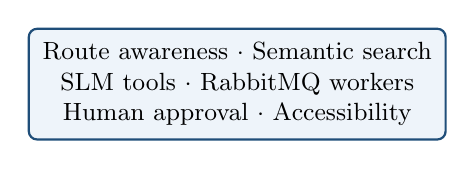
\begin{tikzpicture}
      \node[box, minimum width=4.5cm, minimum height=1.0cm, font=\small] {
        Route awareness $\cdot$ Semantic search\\
        SLM tools $\cdot$ RabbitMQ workers\\
        Human approval $\cdot$ Accessibility
      };
    \end{tikzpicture}

    \column{0.47\textwidth}
    \begin{exampleblock}{The measure of success}
      The system works when travellers feel \emph{in control} of an
      AI-assisted plan — not passengers in an opaque automated workflow.
    \end{exampleblock}
  \end{columns}

  \vspace{0.4cm}
  \centering\small
  Architecture diagrams: Figures~\ref{fig:current-arch}, \ref{fig:future-arch} \quad
  ETL pipeline: Figure~\ref{fig:etl} \quad
  Recommender: Figure~\ref{fig:recommend}\\
  Embedding architecture: Figure~\ref{fig:embedding} \quad
  Chat flow: Figure~\ref{fig:chatflow} \quad
  SLM tools: Figure~\ref{fig:slmworkflow}\\
  RabbitMQ sequence: Figure~\ref{fig:rabbitmq} \quad
  User journey: Figure~\ref{fig:journey} \quad
  Timeline: Figure~\ref{fig:timeline}
\end{frame}

% ============================================================
\begin{frame}[allowframebreaks]{References}
  \tiny
  \begin{thebibliography}{10}

    \bibitem{nielsen1994}
    Jakob Nielsen.
    \newblock \emph{Usability Engineering}.
    \newblock Morgan Kaufmann, 1994.

    \bibitem{shneiderman2016}
    Ben Shneiderman, Catherine Plaisant, Maxine Cohen, Steven Jacobs,
    Niklas Elmqvist, and Nicholas Diakopoulos.
    \newblock \emph{Designing the User Interface: Strategies for Effective
      Human-Computer Interaction}.
    \newblock Pearson, 6th edition, 2016.

    \bibitem{norman2013}
    Don Norman.
    \newblock \emph{The Design of Everyday Things}.
    \newblock Basic Books, revised edition, 2013.

    \bibitem{sweller2011}
    John Sweller, Paul Ayres, and Slava Kalyuga.
    \newblock \emph{Cognitive Load Theory}.
    \newblock Springer, 2011.

    \bibitem{lazar2017}
    Jonathan Lazar, Jinjuan Heidi Feng, and Harry Hochheiser.
    \newblock \emph{Research Methods in Human-Computer Interaction}.
    \newblock Morgan Kaufmann, 2nd edition, 2017.

    \bibitem{dumas1999}
    Joseph Dumas and Janice Redish.
    \newblock \emph{A Practical Guide to Usability Testing}.
    \newblock Intellect Books, revised edition, 1999.

    \bibitem{wcag22}
    W3C Web Accessibility Initiative.
    \newblock \emph{Web Content Accessibility Guidelines (WCAG) 2.2}.
    \newblock World Wide Web Consortium, 2023.

    \bibitem{iso9241}
    ISO.
    \newblock \emph{ISO~9241-11: Ergonomics of Human-System Interaction ---
      Usability: Definitions and Concepts}.
    \newblock International Organization for Standardization, 2018.

    \bibitem{osm}
    OpenStreetMap Contributors.
    \newblock OpenStreetMap Nepal dataset.
    \newblock \url{https://www.openstreetmap.org}, accessed 2026.

    \bibitem{pgvector}
    pgvector: Open-source vector similarity search for PostgreSQL.
    \newblock \url{https://github.com/pgvector/pgvector}, accessed 2026.

    \bibitem{minilm}
    Nils Reimers and Iryna Gurevych.
    \newblock Sentence-BERT: Sentence Embeddings using Siamese BERT-Networks.
    \newblock \emph{EMNLP}, 2019.

    \bibitem{osrm}
    Dennis Luxen and Christian Vetter.
    \newblock Real-time routing with OpenStreetMap data.
    \newblock \emph{ACM SIGSPATIAL}, 2011.

  \end{thebibliography}
\end{frame}

\end{document}
